  % Gemini theme
  % https://github.com/anishathalye/gemini

  \documentclass[final]{beamer}

  % ====================
  % Packages
  % ====================

  \usepackage[T1]{fontenc}
  \usepackage{lmodern}
  \usepackage[size=custom,width=120,height=72,scale=1.0]{beamerposter}
  \usetheme{gemini}
  \usecolortheme{labsix}
  \usepackage{graphicx}
  \usepackage{booktabs}
  \usepackage{tikz}
  \usepackage{pgfplots}
  \usepackage{subfigure}
  \usepackage{amsmath}
  \usepackage{amssymb}

  %%%% Hyperref stuff
  \hypersetup{
    colorlinks  = true, %Colours links instead of ugly boxes
    urlcolor    = cyan, %Colour for external hyperlinks
    linkcolor   = cyan, %Colour of internal links
    citecolor   = red %Colour of citations
  }
  % ====================
  % Maths defs
  % ====================

  \newcommand{\disp}{\omega}					% dispersion parameter
  \newcommand{\chain}{c}							% single transmission chain, integer
  \newcommand{\chains}{\mathbf{C}}		% vector of transmission chains, vector of integers
  \newcommand{\nchains}{K}					  % total number of transmission chains, length of \chains vector
  \newcommand{\ncases}{N}					    % total number of cases, sum of \chains vector

  \newcommand{\seqrate}{\psi}					% proportion of cases that are sequenced
  \newcommand{\nseqs}{J}		          % total number of sequences observed
  \newcommand{\seq}{s}								% single sequence cluster, integer
  \newcommand{\seqs}{\mathbf{S}}			% vector of sequence clusters, vector of integers
  \newcommand{\pr}{\operatorname{Pr}} %% probability

  % ====================
  % Lengths
  % ====================

  % If you have N columns, choose \sepwidth and \colwidth such that
  % (N+1)*\sepwidth + N*\colwidth = \paperwidth
  \newlength{\sepwidth}
  \newlength{\colwidth}
  \setlength{\sepwidth}{0.025\paperwidth}
  \setlength{\colwidth}{0.3\paperwidth}

  \newcommand{\separatorcolumn}{\begin{column}{\sepwidth}\end{column}}

  % ====================
  % Title
  % ====================

  \title{Efficient brute-force marginalisation of discrete variables in Stan: \\
  an epidemic model of sub-critical transmission as a case study}

  \author{Luiz Max Carvalho \inst{1} \and Gytis Dudas \inst{2} \and Andrew Rambaut \inst{3} \and Tanja Stadler\inst{4} \and Trevor Bedford\inst{5}}

  \institute[shortinst]{\inst{1} School of Applied Mathematics, Get\'ulio Vargas Foundation \samelineand \inst{2} Independent consultant \samelineand \inst{3} Institute of Evolutionary Biology, University of Edinburgh \samelineand \inst{4} Department of Biosystems Science and Engineering, ETH Z\"urich  \samelineand \inst{5} Vaccine and Infectious Disease Division, Fred Hutch Cancer Centre}

  % ====================
  % Footer (optional)
  % ====================

  \footercontent{
    \href{https://github.com/maxbiostat/StanCon2020}{https://github.com/maxbiostat/StanCon2020} \hfill
    \href{mailto:lmax.fgv@gmail.com}{lmax.fgv@gmail.com}}
  % (can be left out to remove footer)

  % ====================
  % Logo (optional)
  % ====================

  % use this to include logos on the left and/or right side of the header:
  % \logoright{\includegraphics[height=7cm]{logo1.pdf}}
  % \logoleft{\includegraphics[height=7cm]{logo2.pdf}}

  % ====================
  % Body
  % ====================

  \begin{document}

  \begin{frame}[t]
  \begin{columns}[t]
  \separatorcolumn

  \begin{column}{\colwidth}

  \begin{block}{Motivation}

  As is widely known, the HMC algorithm underlying Stan cannot handle discrete latent variables (parameters).
    Thus, when for one to be able to fit a model containing latent variables in Stan, these need to be marginalised over, either analytically or by brute-force.
  Let $X$ be the discrete latent variables of interest, $\boldsymbol{Y}$ be the data and other variables in the model and $\boldsymbol{\theta}$ be the model parameters.
  We can write
  \[ \pr\left(\boldsymbol{\theta} \mid \boldsymbol{Y} \right ) \propto \sum_{i \in \boldsymbol{\Omega}}  \pr\left(\boldsymbol{\theta} \mid \boldsymbol{Y}, X = i \right) = \sum_{i \in \boldsymbol{\Omega}}  \pr\left(\boldsymbol{Y}, X = i \mid \boldsymbol{\theta} \right)\pi(\boldsymbol{\theta}),\]
  which usually takes the more familiar form
  \begin{equation}
  \label{eq:marginalisation_general}
  \pr\left(\boldsymbol{\theta} \mid \boldsymbol{Y} \right ) \propto \sum_{i=0}^\infty  \pr\left(\boldsymbol{Y}, X = i \mid \boldsymbol{\theta} \right)\pi(\boldsymbol{\theta}).
  \end{equation}
  Here we will discuss a few ways to do the marginalisation in~(\ref{eq:marginalisation_general}) and discuss what is, to the best of our knowledge,~\textbf{a new technique for truncating infinite sums} while controlling approximation error.
  \end{block}

  \begin{block}{A motivating example: sub-critical transmission chains}

  Here are interested in the model~\href{https://journals.plos.org/ploscompbiol/article?id=10.1371/journal.pcbi.1002993}{Blumberg \& Lloyd-Smith, (2013a)},  in which subcritical transmission leads to ``stuttering'' chains of transmission.

  \begin{itemize}
  \item \textbf{Birth-death.}  The model assumes a birth-death process in which an initial single infection results in a distribution of offspring infections.
  \item \textbf{Secondary infection} distribution for each infection follows a negative binomial distribution with mean $R_0$ and over-dispersion parameter $\disp$.
  When $\disp  \to \infty$, the secondary infection distribution is Poisson distributed and when $\disp = 1$  the secondary infection distribution is an exponential distribution.
  \item \textbf{Total number of cases} within a transmission chain, $\chain$, that are caused by a single introduction (including the index case) has limiting distribution:
  \begin{equation}
  \label{eq:R0_pmf}
  \text{Pr}(C = \chain \mid  R_0, \disp) = \frac{\Gamma(\disp \chain + \chain - 1)}{\Gamma(\disp \chain) \Gamma(\chain + 1)} \frac{(R_0/\disp)^{\chain-1}}{(1+R_0/\disp)^{\disp \chain + \chain - 1}}.
  \end{equation}
  \item \textbf{An outbreak} may be comprised of multiple concurrent transmission chains resulting from multiple introduction events.
  Each chain $i$ comprises a count of cases $\chain_i$ and the vector of case counts within distinct transmission chains is $\chains = (\chain_1, \ldots, \chain_\nchains)$.
  \item \textbf{Total number} of cases in the outbreak by $\ncases = \sum_{i=1}^\nchains \chain_i$.
  \item \textbf{MLE.} When $\chains$ are observed directly, the maximum likelihood estimator of $R_0$ is $\widehat{R_0}^{\text{MLE}} = 1 -\frac{K}{N}$.
  % The MLE for $\disp$ is considerably harder to obtain.
  \end{itemize}
  \end{block}
  \end{column}

  \separatorcolumn

  \begin{column}{\colwidth}

  \begin{block}{Modelling observation error}
    The main issue with estimating $\{R_0, \disp\}$ from data is that the clusters (and cluster sizes) are observed imperfectly.
    Here we explore the so-called size-independent model of observation error, which motivates the employment of truncation techniques.

    \heading{Binomial (size-independent) observation error}
      Each  case in chain/cluster $\chain_i$ is observed independently with probability $\seqrate$ such that we now observe a set  $\seqs = (\seq_1, \ldots, \seq_\nseqs)$ of cases.
  Thus we have
  \begin{equation}
  \label{eq:binomial_error}
  P(S = \seq_i \mid  C = \chain_i, \seqrate) = \binom{\chain_i}{\seq_i} \seqrate^{\seq_i} (1-\seqrate)^{\chain_i-\seq_i}.
  \end{equation}
When $s_i = 0$, the cluster is not observed.
The conditional probability that a cluster is not observed is $\text{Pr}(S = 0 \mid C = c_i, \seqrate) = (1-\seqrate)^{c_i}$, while the marginal probability is
\begin{equation}
\label{eq:marg_zero_binomial}
\text{Pr}(S = 0 \mid \seqrate, R_0, \disp) = \sum_{j=1}^\infty \text{Pr}(S = 0 \mid  C = j, \seqrate)  \text{Pr}(C = j \mid R_0, \disp).
\end{equation}
After some manipulation we get
\begin{equation}
\label{eq:summation_weird}
 \sum_{k = 1}^\infty \kappa(k, \disp) b^k = \frac{a}{1 + a},
\end{equation}
with $ a := R_0/\disp$, $b = a/\left(1 + a\right)^{(1+\disp)}$ and $\kappa(\chain, \disp) :=  \frac{\Gamma(\disp \chain + \chain - 1)}{\Gamma(\disp \chain)\Gamma(\chain + 1)}$.
Whilst the mapping $a \mapsto b$ is not invertible analytically, it can be easily inverted numerically~\textit{via} Newton solver.
Hence for the case $s_i = 0$, we can write
\begin{align}
\nonumber
P(S  = 0 \mid R_0, \disp, \seqrate) &=  \sum_{k=1}^\infty  \frac{1 + a}{a} \kappa(k, \disp)b^k (1-\seqrate)^k, \\
\label{eq:probS0}
%  \frac{1 + a}{a} \frac{u}{(1 + u)} =
         &= \frac{\omega + R_0}{R_0} \frac{u}{(1 + u)},
\end{align}
where $b\cdot (1-\seqrate) = u/\left(1 + u\right)^{(1+\disp)}$ and $u$ can be obtained by numerical inversion.
The marginal probability when $S > 0$ is not available in closed-form, and we discuss a strategy to marginalisation in~\textbf{Adaptive truncation}.
      \end{block}

  \begin{alertblock}{Adaptive truncation}
  Let $p(j) := \pr\left(\boldsymbol{\theta} \mid \boldsymbol{Y}, X = j \right)$ let $Q = \sum_{j=s}^\infty p(j)$ be the sum of interest, with $\epsilon$ the desired approximation error.
  Define $L := \lim_{n \to \infty} p(n)$.
  The algorithm can be summarised as follows:
  \begin{enumerate}
  \item Find $\dot{N}$ such that $p(j + 1)/p(j) < 1$ for all $j > \dot{N}$;
  \item  Compute $\dot{Q} = \sum_{j=s}^{\dot{N}} p(j)$;
  \item Let $z_j = \frac{p(j+1) p(j)}{p(j) - p(j + 1)}$;
  \item  Find $\ddot{N} \geq \dot{N}$ such that $p(j) \left( \frac{L}{1-L}\right) + z_j =: \Delta_j < 2\epsilon$ for all $j > \ddot{N}$;
  \item Compute $\ddot{Q} = \sum_{{j^\prime}=\dot{N}}^{\ddot{N}} p(j^\prime)$;
  \item Compute the estimate $\hat{Q} = \dot{Q} + \ddot{Q} + \frac{1}{2}\Delta_{\ddot{N}}$.
  \end{enumerate}
  For the model discussed here, $L = \left[(1 + \disp)/(R_0 + \disp)\right]^{1 + \disp} R_0 (1-\seqrate)$, but usually we have $L=0$.
  \end{alertblock}
  \end{column}

  \separatorcolumn

  \begin{column}{\colwidth}

    \begin{block}{Priors}
     \begin{itemize}
     \item \textbf{Independent priors}.  $\pi(R_0, \disp, \seqrate) = \pi_R(R_0)\pi_H(\disp)\pi_S(\psi)$;
     \item \textbf{Reproduction number}: $\pi_R(R_0)$, $\operatorname{Beta}(1, 1)$ or a boundary-avoiding $\operatorname{Beta}(2, 2)$ -- reference prior is available when $\disp$ is fixed;
     \item \textbf{Dispersion}: $\pi_H(\disp)$, $\operatorname{Gamma}(1, 1)$;
     \item \textbf{Observation probability}: $\pi_S(\psi)$, $\operatorname{Beta}(1, 1)$;
    \end{itemize}

     \heading{Including information about the number of unobserved clusters}

  \begin{itemize}
   \item \textbf{How many unobserved clusters?}
We do not observe the number of size zero clusters, $n_0 = K - J$, directly.
Since we know the number of observed clusters $J$, we can also choose to model the true number of clusters $K$ instead of $n_0$, and this is the route we take here.
   \item\textbf{Marginalising over $K$}
   \begin{itemize}
    \item Let $p_0 := \text{Pr}( S = 0  \mid  R_0, \disp, \seqrate)$;
    \item Then for $k > J$ we have $\text{Pr}(K = k \mid  \boldsymbol\theta) = \text{Pr}(K = k \mid  p_0) = p_0^{k-J}$;
    \item Fix a total (case) count sum: $\ncases = \sum_{i = 1}^K \chain_i$;
    \item Then $K \in [J, U]$, where $U = J + \ncases -T$ and $T= \sum_{i= 1}^J \seq_i$.
   \end{itemize}
Using a doubly-truncated Poisson prior on $K$, the marginalisation is now
\begin{align}
\nonumber
m^{\prime\prime}(J, U, p_0, \lambda_K) &:= \sum_{k = J}^U \text{Pr}(K = k  \mid  p_0) \pi_2(K = k  \mid  \lambda_K) \\
\nonumber
% &= \frac{\exp(\lambda_K(p_0-1)) [F(U ; \lambda_K \cdot p_0) - F(J; \lambda_K \cdot p_0)]}{(F(U; \lambda_K)-F(J; \lambda_K))p_0^J},\\
\label{eq:pois_marg_K}
& = \frac{\exp(\lambda_K(p_0-1))}{p_0^J}.
\end{align}
\end{itemize}
\end{block}

\begin{block}{Prelimnary results}

\begin{center}
\begin{figure}[t!]
\begin{center}
 \hfill
\subfigure[]{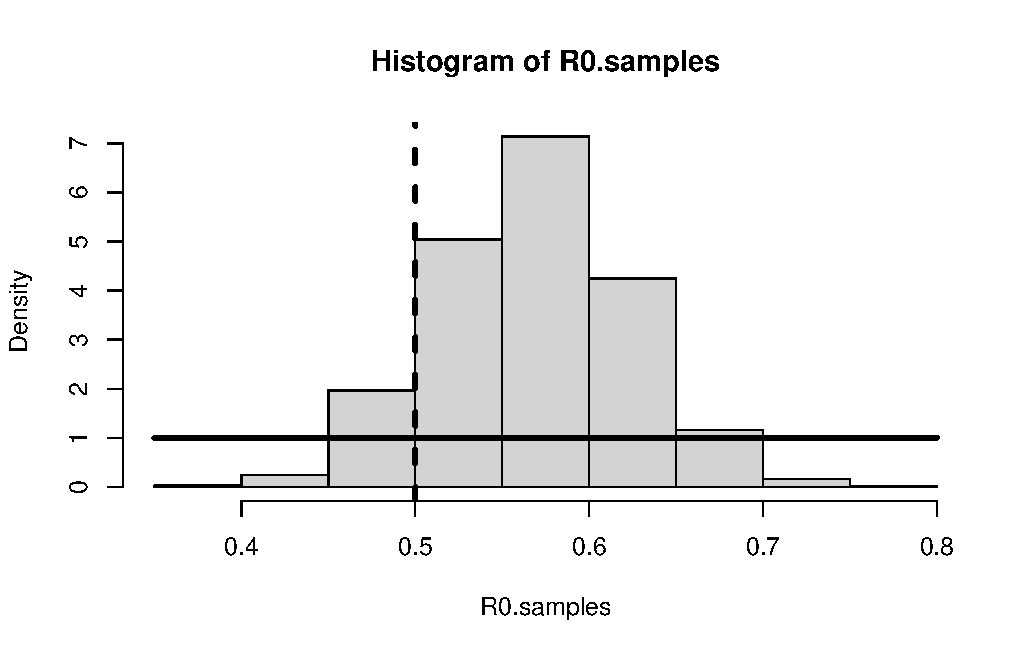
\includegraphics[scale=0.8]{posterior_R0.pdf}}
\hfill
\subfigure[]{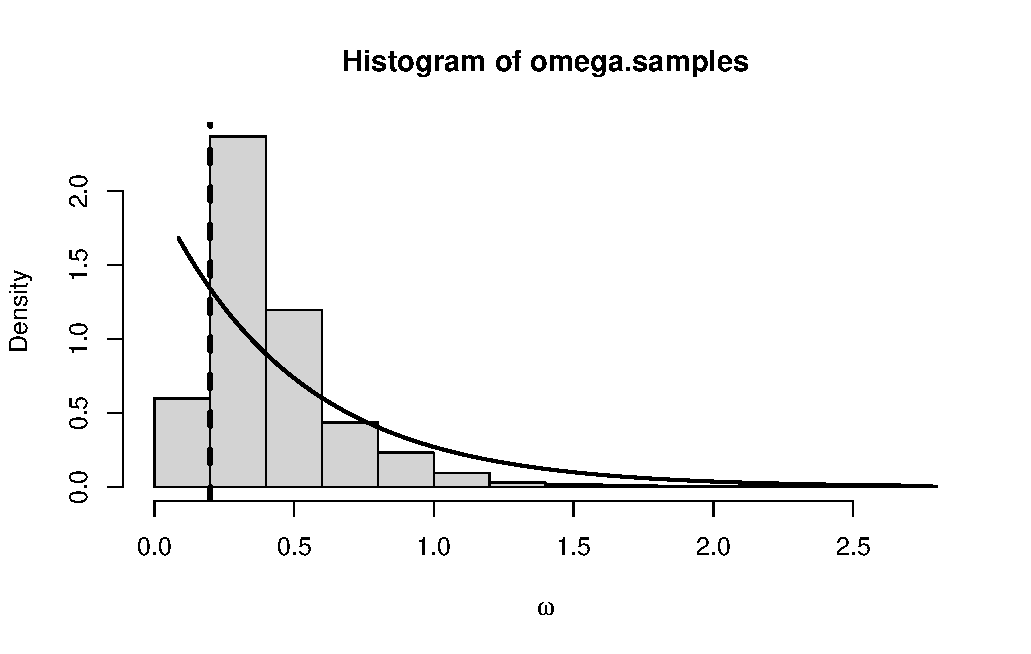
\includegraphics[scale=0.8]{posterior_omega.pdf}}\\
\hfill
\subfigure[]{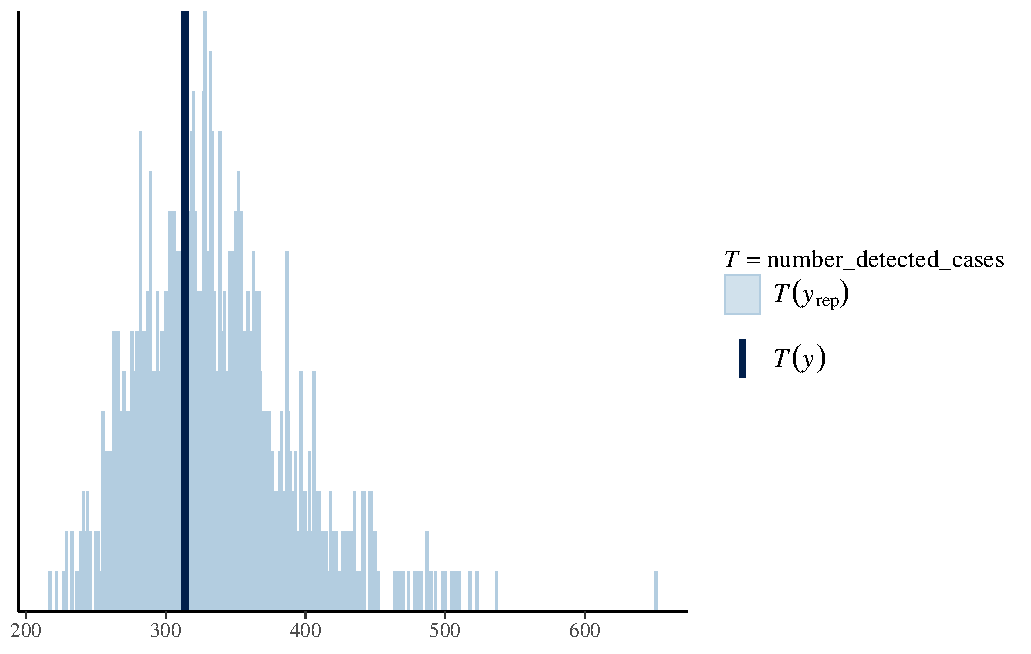
\includegraphics[scale=0.8]{number_detected.pdf}}
\hfill
\subfigure[]{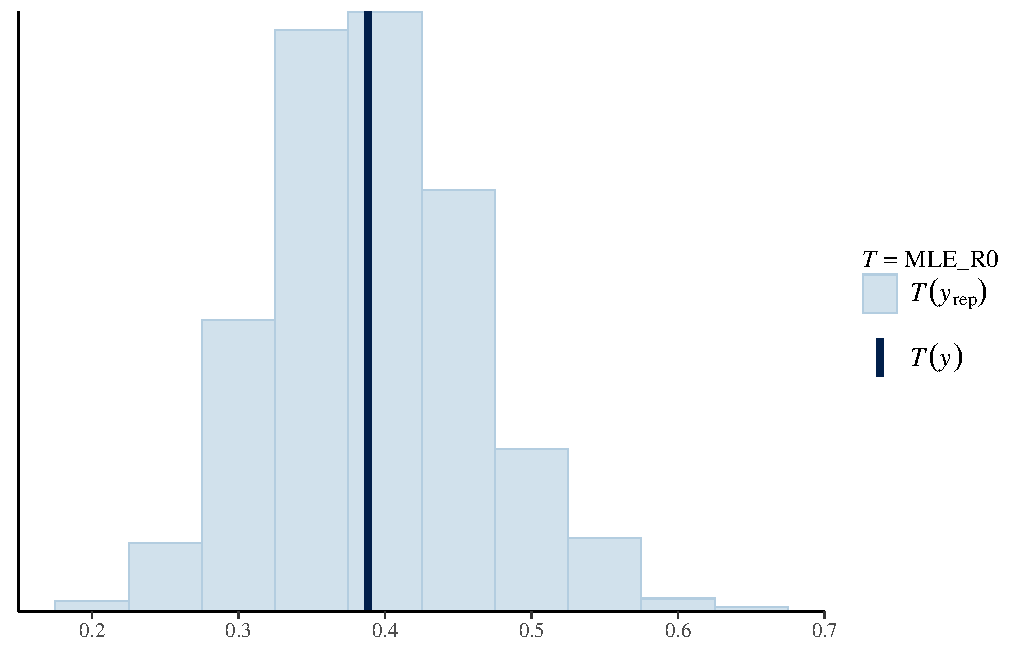
\includegraphics[scale=0.8]{MLE.pdf}}
\hfill
\end{center}

\caption{Posterior distributions and posterior predictives for quantities of interest in the model.}
\end{figure}
\end{center}

\end{block}


  \end{column}

  \separatorcolumn
  \end{columns}
  \end{frame}

  \end{document}
